\chapter{\label{ch:oxview}Structure design and analysis in oxView}

\minitoc

This chapter contains my results on how to design, simulate and analyse DNA and RNA nanostructures. 

%It starts with an introductory description of earlier approaches to this problem and will then describe how my contributions to the oxView tool have improved the previous methods and enabled new results.

As I started this DPhil, I was tasked with the issue of converting origami designs created in caDNAno (see Section~\ref{sec:cadnano}) so that they could be correctly simulated in oxDNA (see Section~\ref{sec:oxDNA}). I soon started collaborating with Hannah Fowler from the Doye group at Theoretical Chemistry, who simulated an extensive collection of old DNA designs. This was a good opportunity to investigate why some structures were more problematic to convert than others.

At this time, the available method for converting a caDNAno design into the oxDNA format was to use an old python script included in the UTILS directory of the oxDNA repository. However, it was not easy to use, and it failed for many structures. At the end of 2018, the tacoxDNA webserver \cite{suma2019tacoxdna} was launched, updating the conversion script and making it more accessible.

Still, since caDNAno structures are drawn on a lattice, where all helices have to be parallel to each other, the resulting oxDNA configurations often had unnaturally extended backbone bonds, requiring time-consuming relaxation.

During a secondment within the {\v{S}}ulc group at Arizona State University in 2019, I contributed to the development of a web-based oxDNA viewer called oxView \cite{poppleton2020design}. Among the main early features that I added to oxView was a cluster-level rigid-body dynamics option (detailed in Section~\ref{sec:rigid-body_dynamics}) that in many cases speed up the relaxation by orders of magnitude compared to oxDNA relaxation alone. Since then, I have collaborated with the {\v{S}}ulc group to add more features and to make the tool more accessible as a visualiser and editor. For our second oxView publication, I rewrote the main parts of the taxoxDNA codebase into TypeScript, resulting in the \emph{taxoxdna.js} library (\url{https://github.com/Akodiat/tacoxdna.js}) which oxView now uses to import various standard design formats (including caDNAno) automatically.

This section will present my own contributions to oxView, unless otherwise stated. However, I also want to acknowledge the work done by Erik Poppleton and Michael Matthies; without them, this tool would not exist. Michael was the original oxView developer and has done great work in supporting live oxDNA relaxations through the \emph{ox-serve} webserver. Erik enabled oxView to render and analyse systems with over a million nucleotides and has created a large set of useful analysis scripts.

\section{Importing designs}
There are a lot of different formats available for DNA origami design; some of the main design tools producing them are covered in Section~\ref{sec:design_tools}. This section will describe how to use oxView to import different designs.

\subsection{Basic import}
Thanks to the \emph{tacoxdna.js} library, importing designs is now generally straightforward. Any loaded structure can then be exported for oxDNA simulation, as described in Section~\ref{sec:oxdna_export}. The formats listed below can all be imported by simply clicking the \emph{Import} button in oxview. However, some additional formats still require the use of the external Tacoxdna webserver \cite{taco}.

\subsubsection{Importing caDNAno files}
JSON files created using caDNAno (described in Section~\ref{sec:cadnano}) can now be imported directly into oxView. See the import dialog shown in Figure~\ref{fig:cadnano_import}.a). First, select the file to import and make sure to also select \emph{caDNAno} as the file format. Next, choose the correct lattice-type; either \emph{Square} or \emph{Hexagonal}. Optionally, input a sequence to assign to the origami scaffold (which will otherwise be random).

\begin{figure}[h]
  \begin{center}
    \begin{overpic}[width=\textwidth]{figures/oxview_import/import.eps}
      \put(-30,810){a)}
      \put(-30,530){b)}
      \put(-30,230){c)}
    \end{overpic}
    \caption{Importing caDNAno structues into oxView. a) The tacoxdna.js library import dialog in oxView (left), seen here importing a caDNAno design. Note the web browser console shown to the right, where any additional output from the import is written. b) Imported linear actuator rail design from \cite{benson2021strategies}. c) Complete linear actuator structure from \cite{benson2021strategies} assembled in oxView, after also importing the slider caDNAno design.}
    \label{fig:cadnano_import}
  \end{center}
\end{figure}

Another option is to use the tacoxdna webservice to convert the caDNAno design into oxDNA files and then load those into oxView. However, designs loaded directly into oxView have the benefit of including correct colouring, clustering and base-pairing information, which would otherwise have been lost.

\subsubsection{Importing rpoly files}
Rpoly files are the output from the BSCOR \cite{vHelix} tool (described in Section~\ref{sec:bscor}) for converting polyhedral meshes into DNA origami.
Select the rpoly file to import, making sure that \emph{rpoly} is selected as the file format. Optionally, input a sequence to assign to the origami scaffold (which will otherwise be random).

\subsubsection{Importing Tiamat files}
Select the Tiamat \emph{.dnajson} file to import, making sure that \emph{tiamat} is selected as file format. Binary \emph{.dna} Tiamat files need to be reopened in Tiamat and saved to the text-based \emph{.dnajson}. Select Tiamat version (1 or 2), then select the nucleic acid type (DNA or RNA).

By default, nucleotides without assigned base types will be given a random type. However, it is also possible to select a fixed default base.

\subsubsection{Importing PDB files}
While I did include the DNA PDB to oxDNA converter from Tacoxdna in \emph{tacoxdna.js}, a more versatile PDB import was created by Jonah Procyk to support his ANM-oxDNA model \cite{procyk2021coarse}. Simply drag and drop (or load) a PDB file into an oxView window and the DNA, RNA and/or protein it contains will be automatically converted and loaded.

%The simplest method is now to use the recently published tacoxDNA web service \cite{suma2019tacoxdna} (whose conversion script is more or less the same as in the oxDNA repository). However, the script can still fail to parse some designs, so a future implementation that uses the native caDNAno library for parsing would be preferable.

\subsection{Multi-component designs}
Designs spread across multiple files (or even multiple design tools) can be easily combined in oxView by simply importing them all and using the editing tools to arrange and connect them properly.

\subsection{Far-from-physical caDNAno designs}
Some structures, while converted without failure to the oxDNA format, will have a very far-from-physical configuration due to the way they are drawn in caDNAno. As mentioned above, since it is only possible to draw all helices parallel to each other (on a lattice), backbone bonds may be very elongated, creating high energies and/or topological problems.

The oxDNA software already includes relaxation procedures for such structures, bringing them together in a slow and controlled manner using a specified maximum backbone force. However, for large structures, this can take a very long time, even while using GPU simulation.

In such cases, another software I have investigated, called mrdna (Multi-resolution DNA nanotechnology), proves very useful \cite{maffeo2018}. It is a python package using ARBD (Atomic Resolution Brownian Dynamics), both being developed by Chris Maffeo, to simulate double- and single-stranded DNA structures at multiple levels of coarse-graining. Since these simulations are more coarse-grained than oxDNA, they run significantly faster. Furthermore, after I have been in contact with Chris, mrdna can now also be configured to output and simulate oxDNA configurations as the final simulation step. Because of this, mrdna can also be useful for converting simple structures if tacoxDNA fails to parse the caDNAno file.

\section{Rigid-body manipulation and dynamics}
\label{sec:rigid-body_dynamics}
Rapid relaxation of converted cadnano designs

Rigid-body manipulation \cite{huang2019uncertainty}. The translation and rotation tools in oxView allow users to select and rearrange blocks of nucleotides as rigid bodies. 

Dynamics \cite{baraff1997introduction}

Manually, on import or through DBSCAN algorithm \cite{ester1996density}.

Clusters held together with spring forces at each shared backbone bond, with a magnitude of 
$$ f_{\rm spr} = c_{spr}(l - l_r),$$
where \(c_{spr}\) is a spring constant, \(l\) is the current bond length and \(l_r\) is the relaxed bond length. To avoid overlaps, a simple linear repulsive force, of magnitude
$$ f_{\rm rep} = max\left(c_{rep}\left(1-\frac{d}{r_a+r_b}\right),0\right)$$ is added between the centre of each group, where \(c_{rep}\) is a repulsion constant, \(d\) is the distance between the two centres of mass, and \(r_a+r_b\) is the sum of the group radii (the greatest distance they can be while still overlapping).

As seen in Figure~\ref{fig:rigidBody},

\begin{figure}[h]
  \centering
  \begin{overpic}[width=\textwidth]{figures/icosahedron.png}
    \put(0,300){a)}
    \put(240,300){b)}
    \put(620,300){c)}
  \end{overpic} 
  \caption{Rigid-body dynamics of clusters. Snapshots from the automatic rigid-body relaxation of an icosahedron, starting with the configuration converted from caDNAno \textbf{a)}, through the intermediate \textbf{b)} where the dynamics are applied, and \textbf{c)} the final resulting relaxed state.}
  \label{fig:rigidBody}
\end{figure}

\section{Editing designs}

\begin{figure}[h]
\begin{overpic}[width=\textwidth]{figures/tetra.eps}
  \put(0,200){a)}
  \put(200,200){b)}
  \put(470,200){c)}
  \put(740,200){d)}
\end{overpic}
\caption{Designing the DNA tetrahedron from \cite{goodman2005rapid} using the oxView editing tools. a) An initial 20 base pair helix created. b) Duplicated helices being rotated and translated into place. c) Strands ligated together. d) The resulting 3D tetrahedron shape, as seen after applying rigid-body dynamics.}
\label{fig:design}
\end{figure}

While oxView started as a visualisation tool, it has since been extended with a number of editing features. One of the earliest was the ability to perform rigid-body manipulation of selected nucleotides by dragging them with the mouse. I contributed by adding transformation gizmos that simplify translation and rotation of selections using on-screen arrows and arcs for the user to manipulate. See Table~\ref{table:edit_tools} for a complete list of the editing tools currently available in oxView.

With the ability to create, remove, connect, and disconnect nucleotides, oxView users can now design structures from scratch. See, for example, Figure~\ref{fig:design}, where the DNA tetrahedron from \cite{goodman2005rapid} is created. The user first creates an initial helix (Figure~\ref{fig:design}.a) by typing a 20-base sequence and clicking the ``Create'' button in the ``Edit'' tab. Note that the ``Duplex mode'' need to be active in order for the complementary strand to be created automatically. Next, the user can copy and paste the helix repeatedly, using the ``Translate'' and ``Rotate'' tools to position the helices as seen in~\ref{fig:design}.b).

The do/undo system

%ligate, nick, do/undo, extend and create strands

\newcommand{\toolHeight}{1.5em}


\begin{table}[h]
\centering

\begin{tabularx}{\textwidth} { >{\centering\arraybackslash}m{3em} | X }
 \hline
 Tool & Description \\ [0.5ex] 
 \hline
 \hline
\includesvg[height=\toolHeight]{figures/tools/create} & \textbf{Create} a new strand from a given sequence. Select \textit{duplex mode} to instead create a helix. \\ \hline
\includesvg[height=\toolHeight]{figures/tools/copy} & \textbf{Copy} the selected elements (Ctrl+C). \\ \hline
\includesvg[height=\toolHeight]{figures/tools/cut} & \textbf{Cut} the selected elements (Ctrl+X). \\ \hline
\includesvg[height=\toolHeight]{figures/tools/paste} & \textbf{Paste} elements from clipboard (Ctrl+V to paste in original position, or Ctrl+Shift+V to paste in front of camera). \\ \hline
\includesvg[height=\toolHeight]{figures/tools/delete} & \textbf{Delete} all currently selected elements (delete). \\ \hline
\includesvg[height=\toolHeight]{figures/tools/ligate} & \textbf{Ligate} two strands by selecting the 3' and 5' endpoint elements to connect (L). \\ \hline
\includesvg[height=\toolHeight]{figures/tools/nick} & \textbf{Nick} a strand at the selected element (N) \\ \hline
\includesvg[height=\toolHeight]{figures/tools/extend} & \textbf{Extend} strand from the selected element with the given sequence. Select \textit{duplex mode }to also extend the complementary strand. \\ \hline
\includesvg[height=\toolHeight]{figures/tools/insert} & \textbf{Insert} (add) elements within a strand after the selected element. \\ \hline
\includesvg[height=\toolHeight]{figures/tools/skip} & \textbf{Skip} (remove)  selected elements within a strand. \\ \hline
\includesvg[height=\toolHeight]{figures/tools/rotate} & \textbf{Rotate} selected elements around their center of mass (R). \\ \hline
\includesvg[height=\toolHeight]{figures/tools/translate} & \textbf{Translate} currently selected elements (T). \\ \hline
\includesvg[height=\toolHeight]{figures/tools/moveto} & \textbf{Move to}. Move other selected elements to the position of the most recently selected element. \\ \hline
\includesvg[height=\toolHeight]{figures/tools/connect3s} & \textbf{Connect 3' duplex}. Connects the 3' ends of two selected staple strands with a duplex, generated from the sequence input. \\ \hline
\includesvg[height=\toolHeight]{figures/tools/connect5s} & \textbf{Connect 5' duplex}. Connects the 5' ends of two selected staple strands with a duplex, generated from the sequence input. \\ \hline
\includesvg[height=\toolHeight]{figures/tools/set} & \textbf{Set} the sequence of currently selected elements. Select duplex mode to also set the complementary sequence on paired elements. \\ \hline
\includesvg[height=\toolHeight]{figures/tools/get} & \textbf{Get}. Assigns the sequence of selected bases to the sequence input.  \\ \hline
\includesvg[height=\toolHeight]{figures/tools/rc} & \textbf{Reverse complement}. Generates the reverse complement of a provided sequence. \\ \hline
\includesvg[height=\toolHeight]{figures/tools/search} & \textbf{Search}. Highlights the position the provided sequence in each strand, if present. \\ \hline
\end{tabularx}

\caption{Editing tools available in oxView}
\label{table:edit_tools}
\end{table}



\section{Visualization options}
Depending on the design, a user of oxView might want to modify the visualisation settings to make certain features of the structure more or less visible.

\paragraph{Centring with periodic boundary conditions} A useful utility when visualising an oxDNA trajectory is to keep the structure centred at the origin, stopping it from drifting out of view. The method described in \cite{PBC_centring} was used to achieve centring while taking periodic boundary conditions into account.

% https://doi.org/10.1080/2151237X.2008.10129266
% https://en.wikipedia.org/wiki/

In essence, for each coordinate \(p_j = \left(p_x^j, p_y^j, p_z^j\right) \) in the centring set of size \(n\), each dimension \(i \in \left\{x,y,z\right\}\) gets averaged in its own variable \(\alpha_i\), representing its 1D interval as a 2D circle (where the circumference \(b_i\) is the bounding box side length:

\[
  c_i = \frac{1}{n} \sum_{j = 1}^{n} \left[ \cos \left( \alpha_i^j \right), \sin \left( \alpha_i^j \right) \right]  
\]

Where \(\alpha_i^j = \frac{2 \pi}{b_i} p_i^j\) is the angle on the unit circle and \(c_i\) is the average 2D position representing dimension \(i\). Finally, the averages are converted back to cartesian coordinates:

\[
  cm_i = \pi + \frac{b_i}{2\pi} atan2(-c_{i,y}, -c_{i, x})
\]

\paragraph{Change component sizes}


, change colours, fog, virtual reality.

\begin{figure}[h]
\centering\includegraphics[width=\textwidth]{figures/oxview.png} 
\caption{Screenshot of the online oxView tool, exporting a video of a slider on a rail from a simulated trajectory.}
\label{fig:oxview}\end{figure}

\section{Exporting designs}
\label{sec:oxdna_export}
Once a structure has been created in or loaded into oxView, it can be exported in a variety of formats.

\subsection{Exporting oxDNA simulation files}
OxView can export topology, configuration, and external force files for oxDNA simulation. Simply click the ``Export oxDNA'' button in the ``File'' menu and select the required file types.

One important thing to note is that the oxDNA format requires nucleotides to be correctly sorted with consecutive indices. Furthermore, this sorting is done, against convention, in a 3' to 5' order. Meanwhile, to facilitate editing, oxView nucleotides keep their indices even if the topology changes. Thus, nucleotides indices may be reassigned on oxDNA export, so it is important to export all files (topology, configuration, and forces) if the design has been edited.

\subsection{Exporting other 3D formats}
File formats such as glTF and STL contain geometrical information that can be 3D printed or imported into other 3D software such as Blender. OxView exports the scene as it is at the moment of export (at the current frame if a simulation trajectory is loaded), so it is important to configure intended component sizes and colours beforehand.

STL is an old and common standard for 3D shapes, containing only vertex coordinates (no colours). It is a popular input for 3D printing, but the file size is relatively large.

The glTF format (or glb if binary) is a modern standard for 3D scenes, storing geometry, hierarchy, and even material properties.

\subsection{Exporting sequence files}
Strand sequences can be exported as standard CSV files using the ``Sequence file'' export button in the ``File'' tab. The designed sequences can then be ordered and assembled experimentally.

\subsection{Saving image files}\label{sec:image_export}

It is possible to save an image of the current oxView view by simply clicking the ``Save image'' button in the ``File'' tab. This is a preferred option over a screenshot for two reasons. First, it is possible to increase the resolution by a scaling factor found in the ``Image size'' dropdown (rescale the browser window to change the aspect ratio of the image). Secondly, the background of the saved image will be transparent, simplifying further editing and composition.

For cover art and photo-realistic renders, it is also possible to export and load a glTF file into (for example) Blender, as seen in Figure~\ref{fig:image_export}. Note that in current Blender versions (2.9), large structures take a long time to import. So, make sure to disable any components not needed before export.

\begin{figure}[h]
  \centering
  \begin{overpic}[width=\textwidth]{figures/oxview_image_export/row.png}
    \put(0,280){a)}
    \put(320,280){b)}
    \put(670,280){c)}
  \end{overpic}
  \caption{Component scaling and image export. a) Default oxView visualisation. b) Custom component scale and visibility. Using the``Visible components'' dropdown in the ``View'' menu,  the backbone spheres have been scaled up by a factor of 4.18 while all other nucleotide components have been hidden. c) The scaled scene in b) exported as glTF and rendered using Cycles in Blender.}
  \label{fig:image_export}
\end{figure}

\subsection{Creating videos}
One of the earlier features I implemented in oxView was the ability to create videos from oxDNA simulation trajectories. It is also possible to create lemniscate videos of single configurations, where the camera moves around the structure in a lemniscate-shaped loop. The video export uses the \texttt{CCapture.js} library, grabbing the \texttt{Three.js} canvas and outputting either ``webm'' or ``gif'' animations, or each frame as separate ``jpg'' or ``png'' images.

Click ``Create video'' in the ``File'' menu, choose video type (trajectory or lemniscate), file format, and frame rate. For lemniscate videos, it is also possible to set a video duration.

For trajectory videos, the camera can be manually moved while the video is being recorded, thus showing the simulation from different angles.

Another option for video creation is to follow the steps described in Section~\ref{sec:image_export}. When the structure is loaded into Blender, the camera can be animated (or the design rotated) using keyframes to render high-quality videos. To render an oxDNA simulation, use the ``traj2blender.py'' script, found at \url{https://github.com/Akodiat/traj2blender}, to automatically load keyframes corresponding to simulation steps.

\section{Converting RNA origami designs}
\label{sec:converting_rna_origami}
During my secondment at the Andersen lab in Aarhus, I worked with converting RNA structures designed using their ASCII-based blueprint format into oxRNA simulation files. Examples of converted structures are shown in Figure~\ref{fig:oxRNA_sims}. The Andersen lab already has scripts, soon to be published, for parsing their blueprint files and building the corresponding PDB structures (the first two columns of Figure~\ref{fig:oxRNA_sims}). However, the resulting PDB files are not relaxed and would take a long time to relax using all-atom simulation. As such, I modified the tacoxDNA \cite{suma2019tacoxdna} PDB parser to enable PDB-to-oxRNA conversion. I have contacted Lorenzo to let him know about these additions, and hopefully, they will be included in a future version of tacoxDNA. One issue I noticed with the conversion was that the asterisk (*) and prime (') characters were used interchangeably in the RNA motif library to name atoms of the sugar group, causing problems with the tacoxDNA script, which only recognises the prime. This has already been fixed in tacoxDNA. The third column of Figure~\ref{fig:oxRNA_sims} shows the structures relaxed and simulated in oxRNA, some significantly different from the previously available PDB models in the second column.

% "The asterisk (*) is used in place of the prime character (') for naming atoms of the sugar group" - https://cdn.rcsb.org/wwpdb/docs/documentation/file-format/PDB_format_1996.pdf

\begin{figure}[h]
\begin{center}
\makebox[\textwidth][c]{a)  
  \centering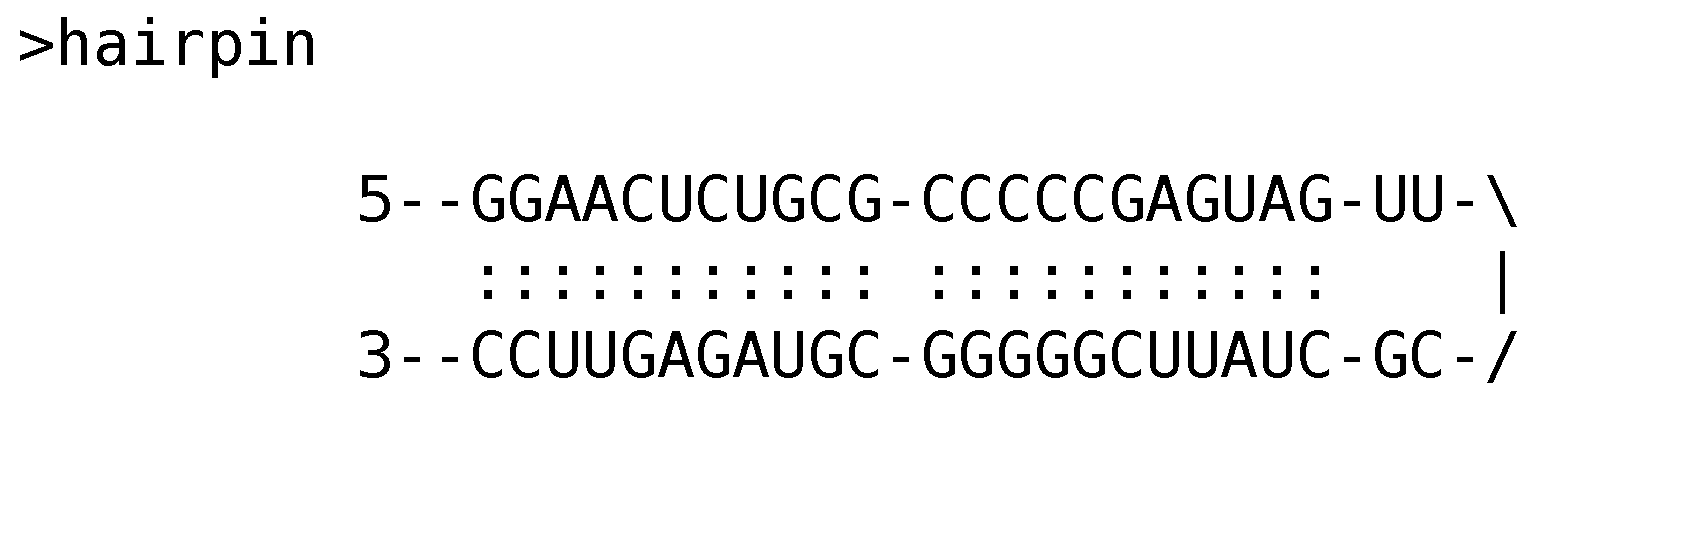
\includegraphics[align=c,width=\textwidth/3]{figures/oxrna_sims/hairpin.eps} \centering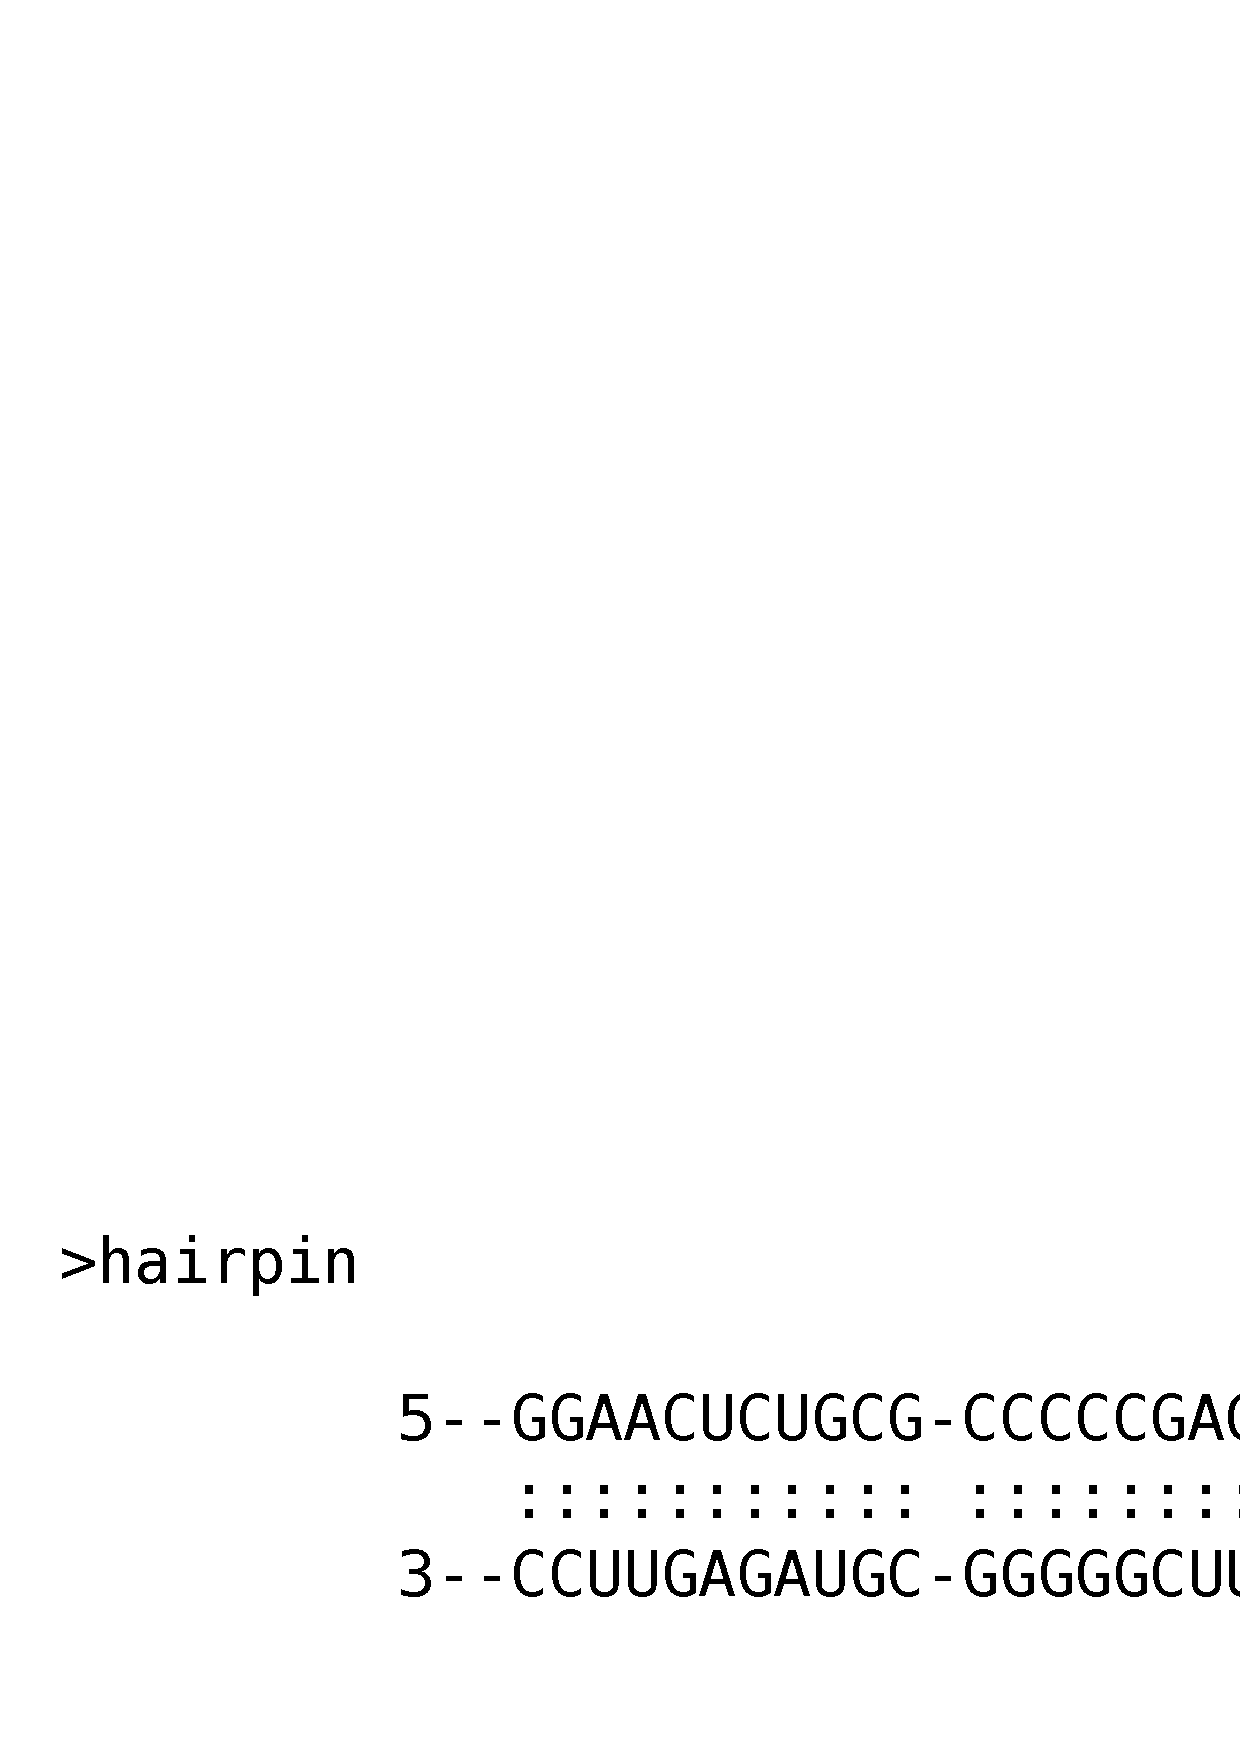
\includegraphics[align=c,width=\textwidth/3]{figures/oxrna_sims/hairpin.png} \centering\includegraphics[align=c,width=\textwidth/3]{figures/oxrna_sims/hairpin_last_conf.png}
}
\makebox[\textwidth][c]{b)  
  \centering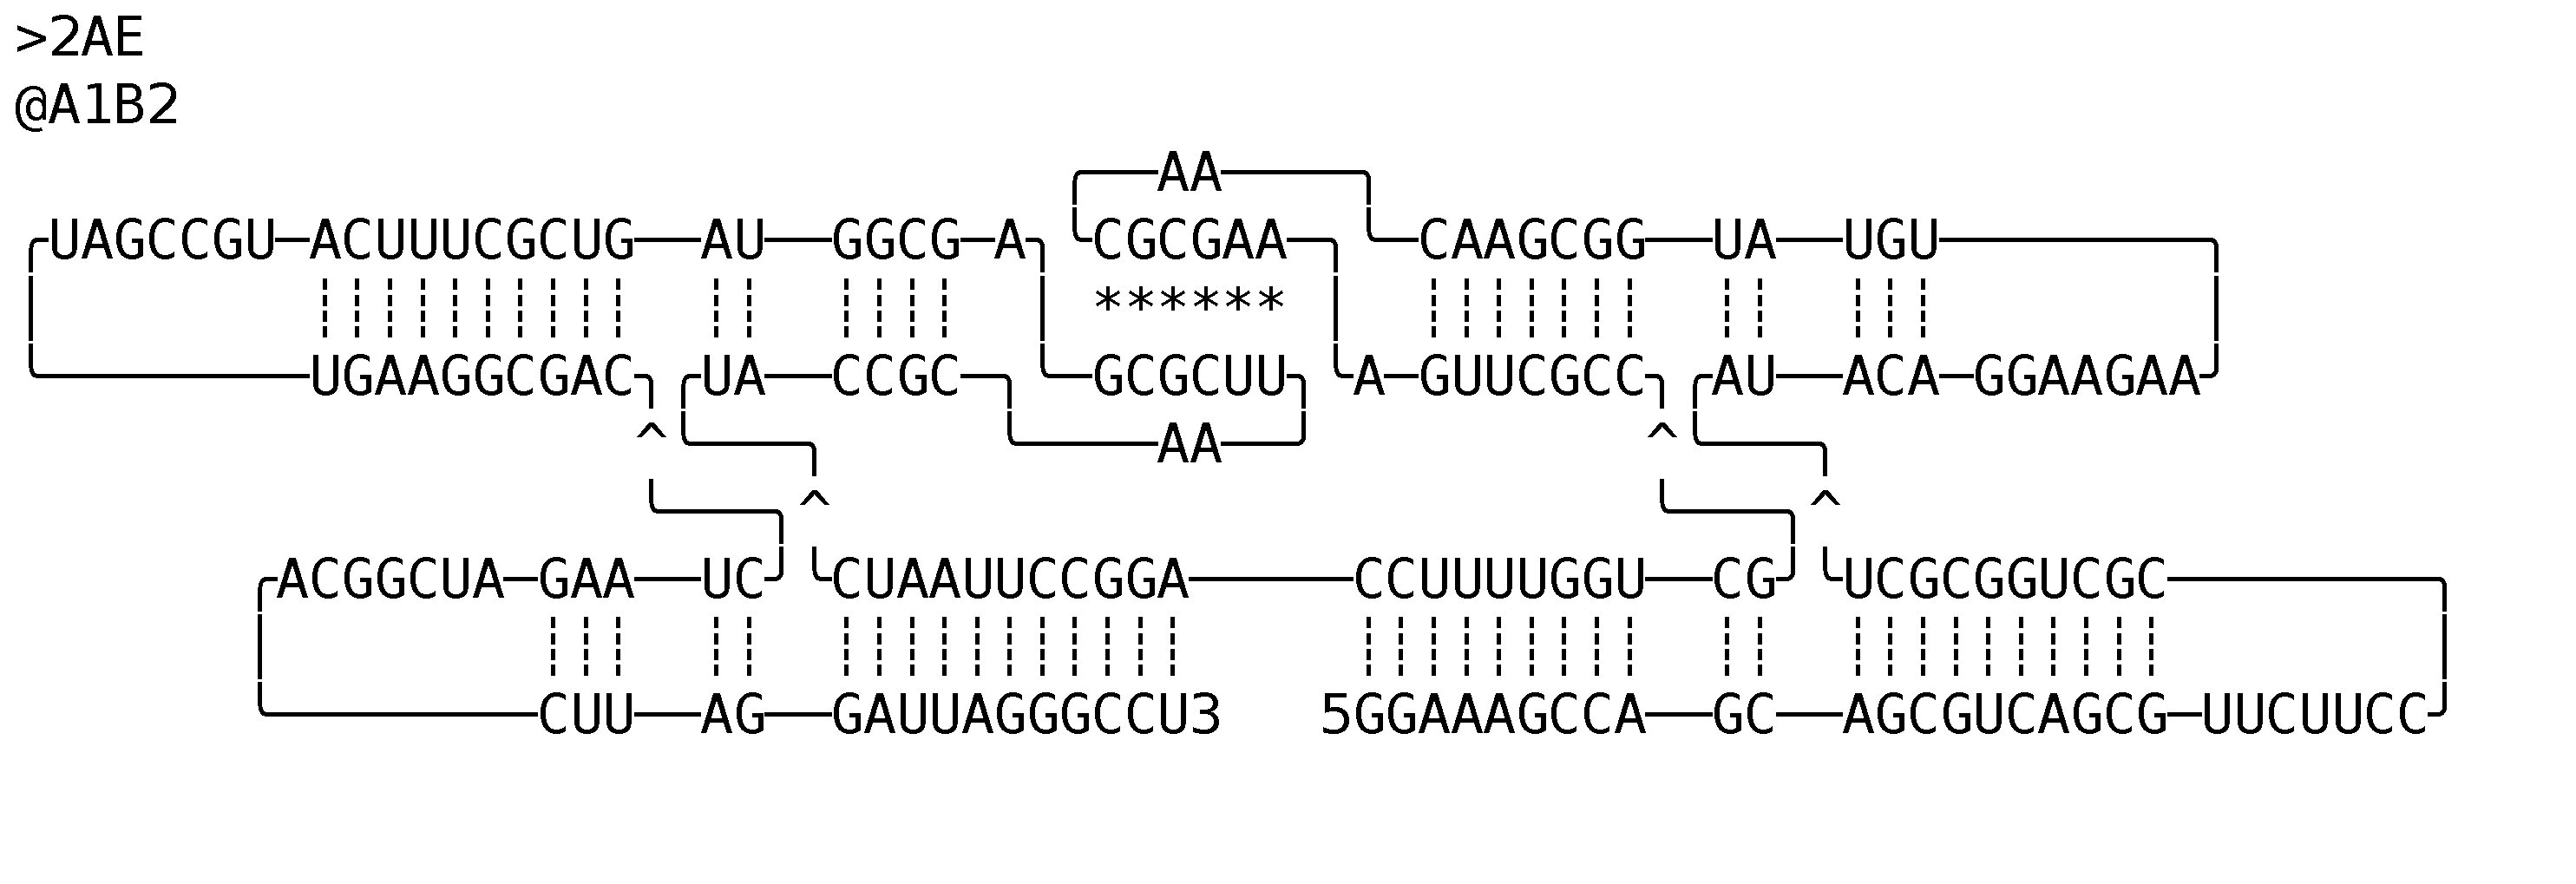
\includegraphics[align=c,width=\textwidth/3]{figures/oxrna_sims/2AE.eps} \centering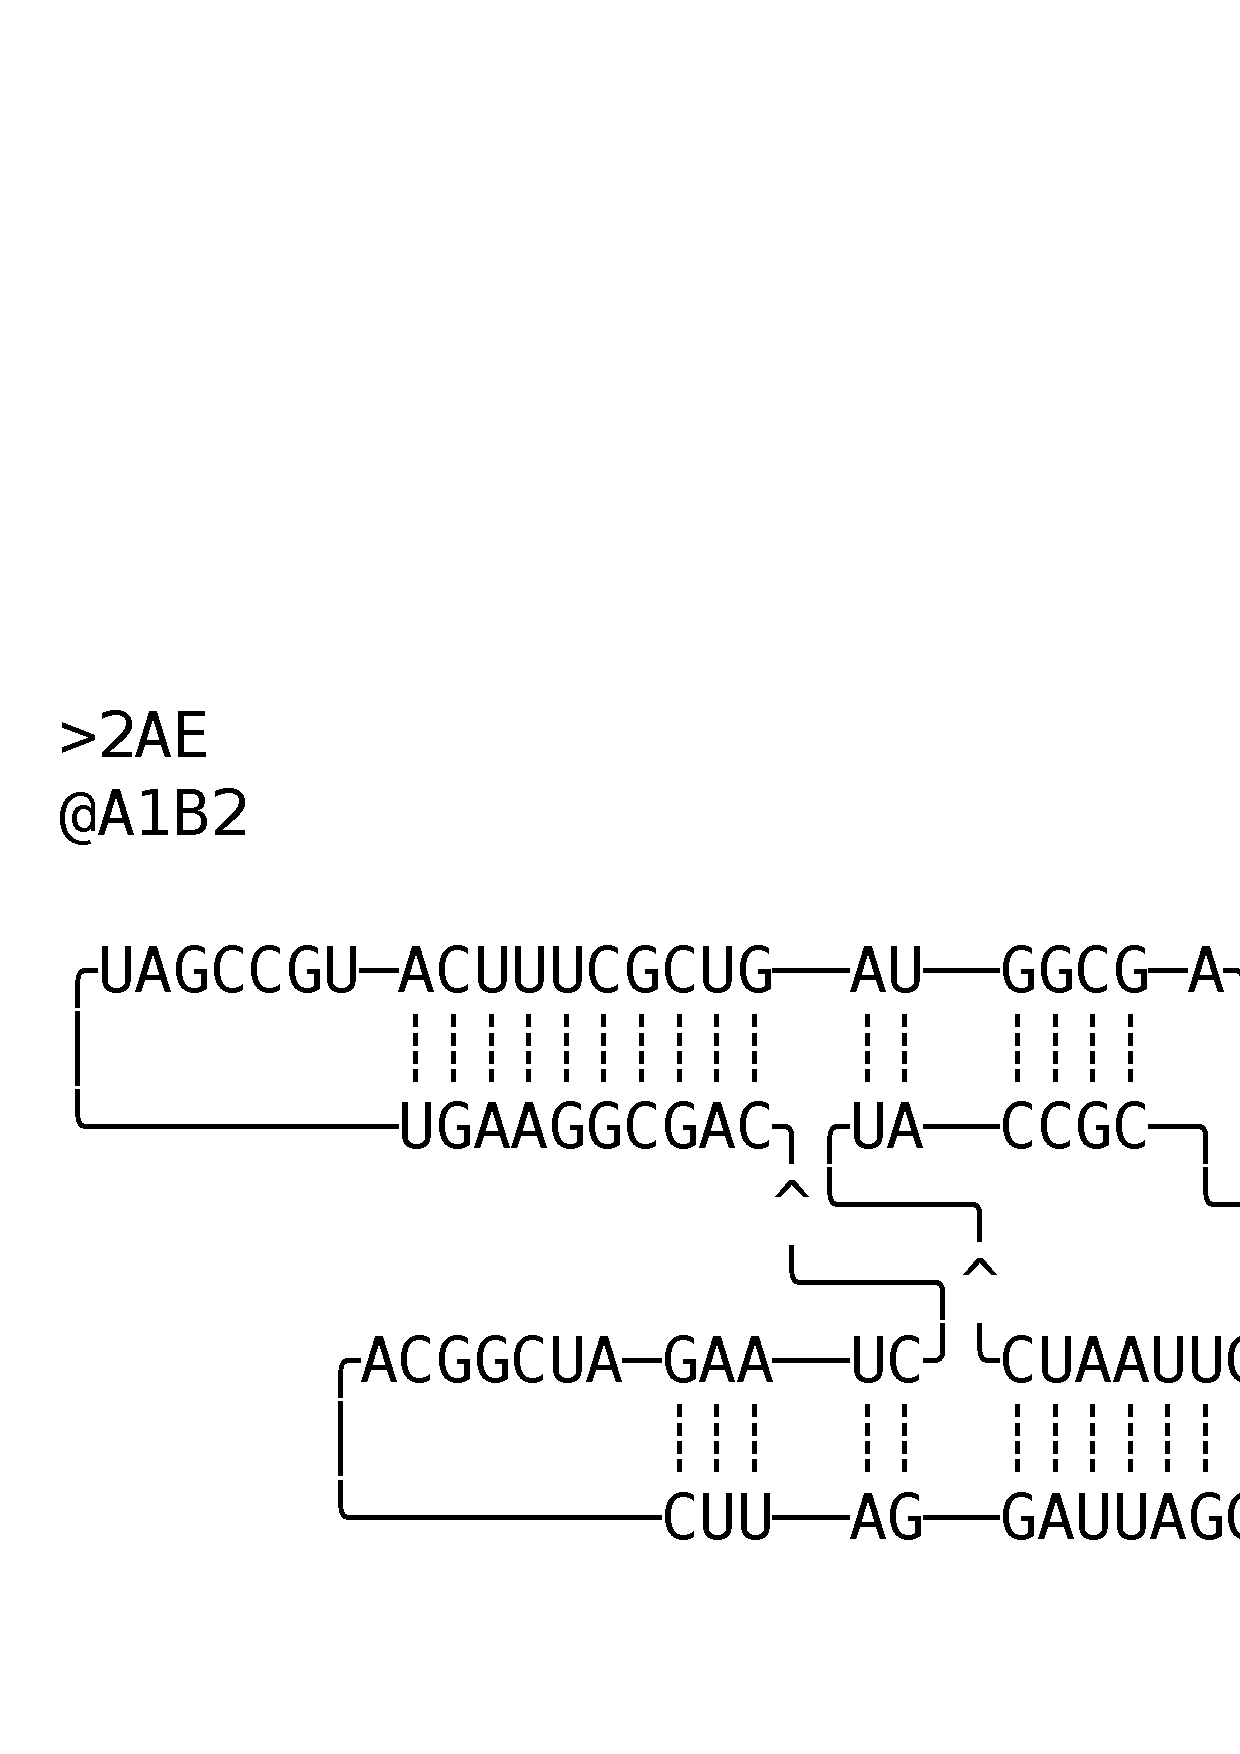
\includegraphics[align=c,width=\textwidth/3]{figures/oxrna_sims/2AE.png} \centering\includegraphics[align=c,width=\textwidth/3]{figures/oxrna_sims/2AE_last_conf.png}
}
\makebox[\textwidth][c]{c) 
  \centering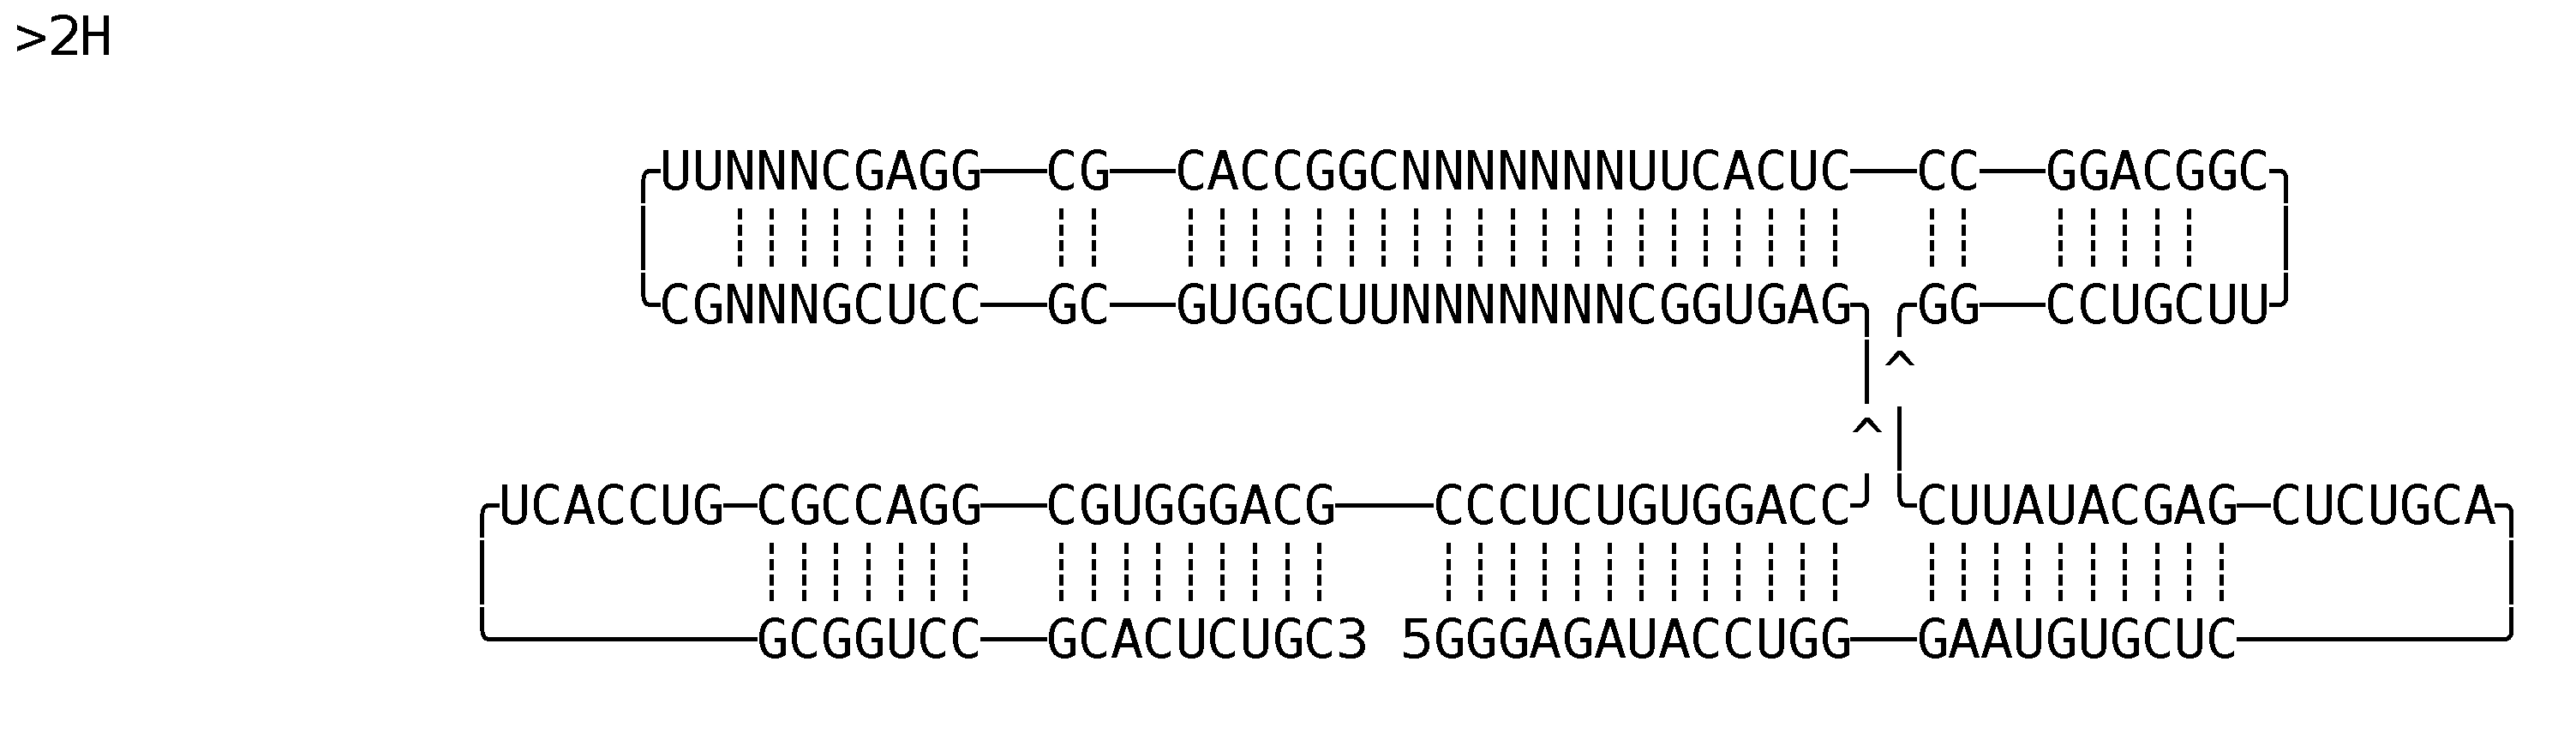
\includegraphics[align=c,width=\textwidth/3]{figures/oxrna_sims/2H.eps} \centering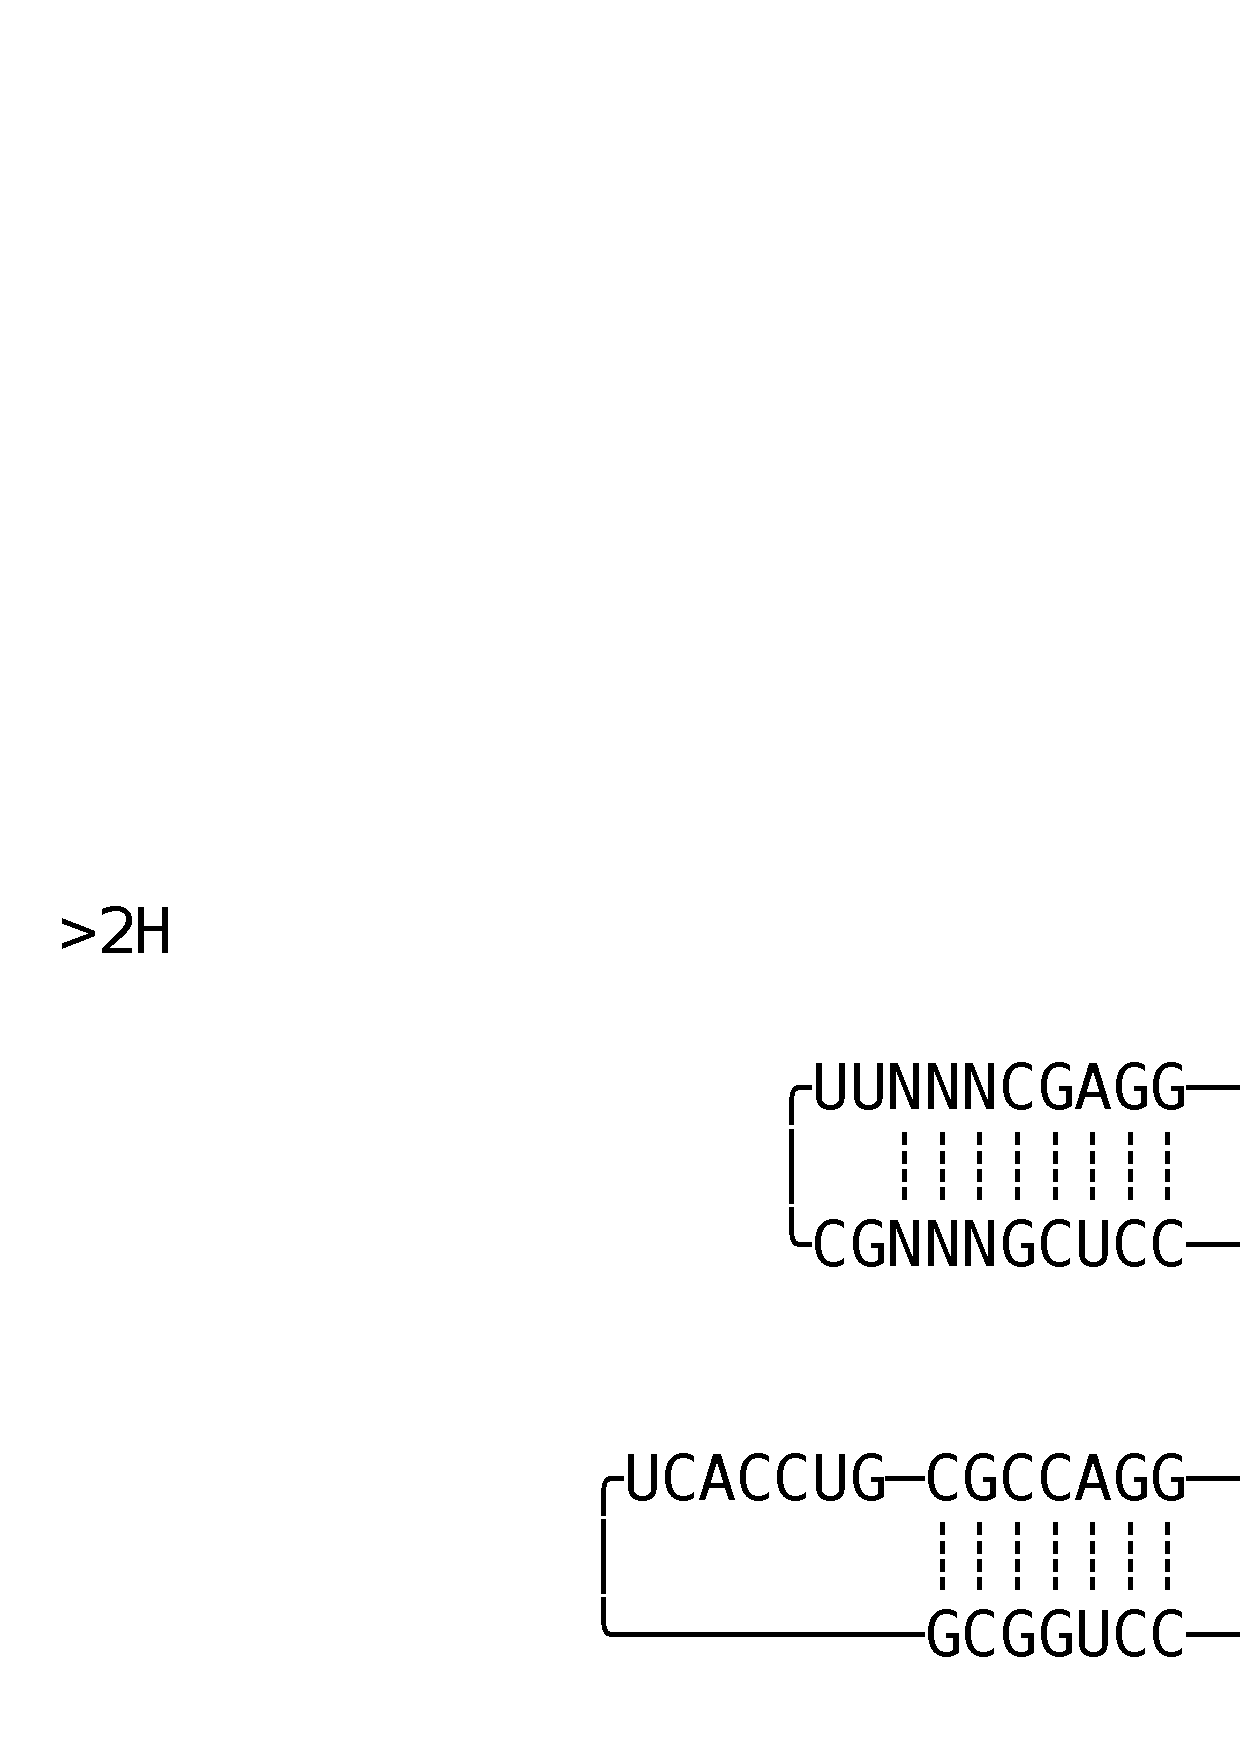
\includegraphics[align=c,width=\textwidth/3]{figures/oxrna_sims/2H.png}
  \centering\includegraphics[align=c,width=\textwidth/3]{figures/oxrna_sims/2H_last_conf.png}
}
\makebox[\textwidth][c]{d) 
  \centering\includegraphics[align=c,width=\textwidth/3]{figures/oxrna_sims/3H-Tri6.eps} \centering\includegraphics[align=c,width=\textwidth/3]{figures/oxrna_sims/3H-Tri6_pre.png}
  \centering\includegraphics[align=c,width=\textwidth/3]{figures/oxrna_sims/2H-Tri6_tri.png}
}
\makebox[\textwidth][c]{e)  
  \centering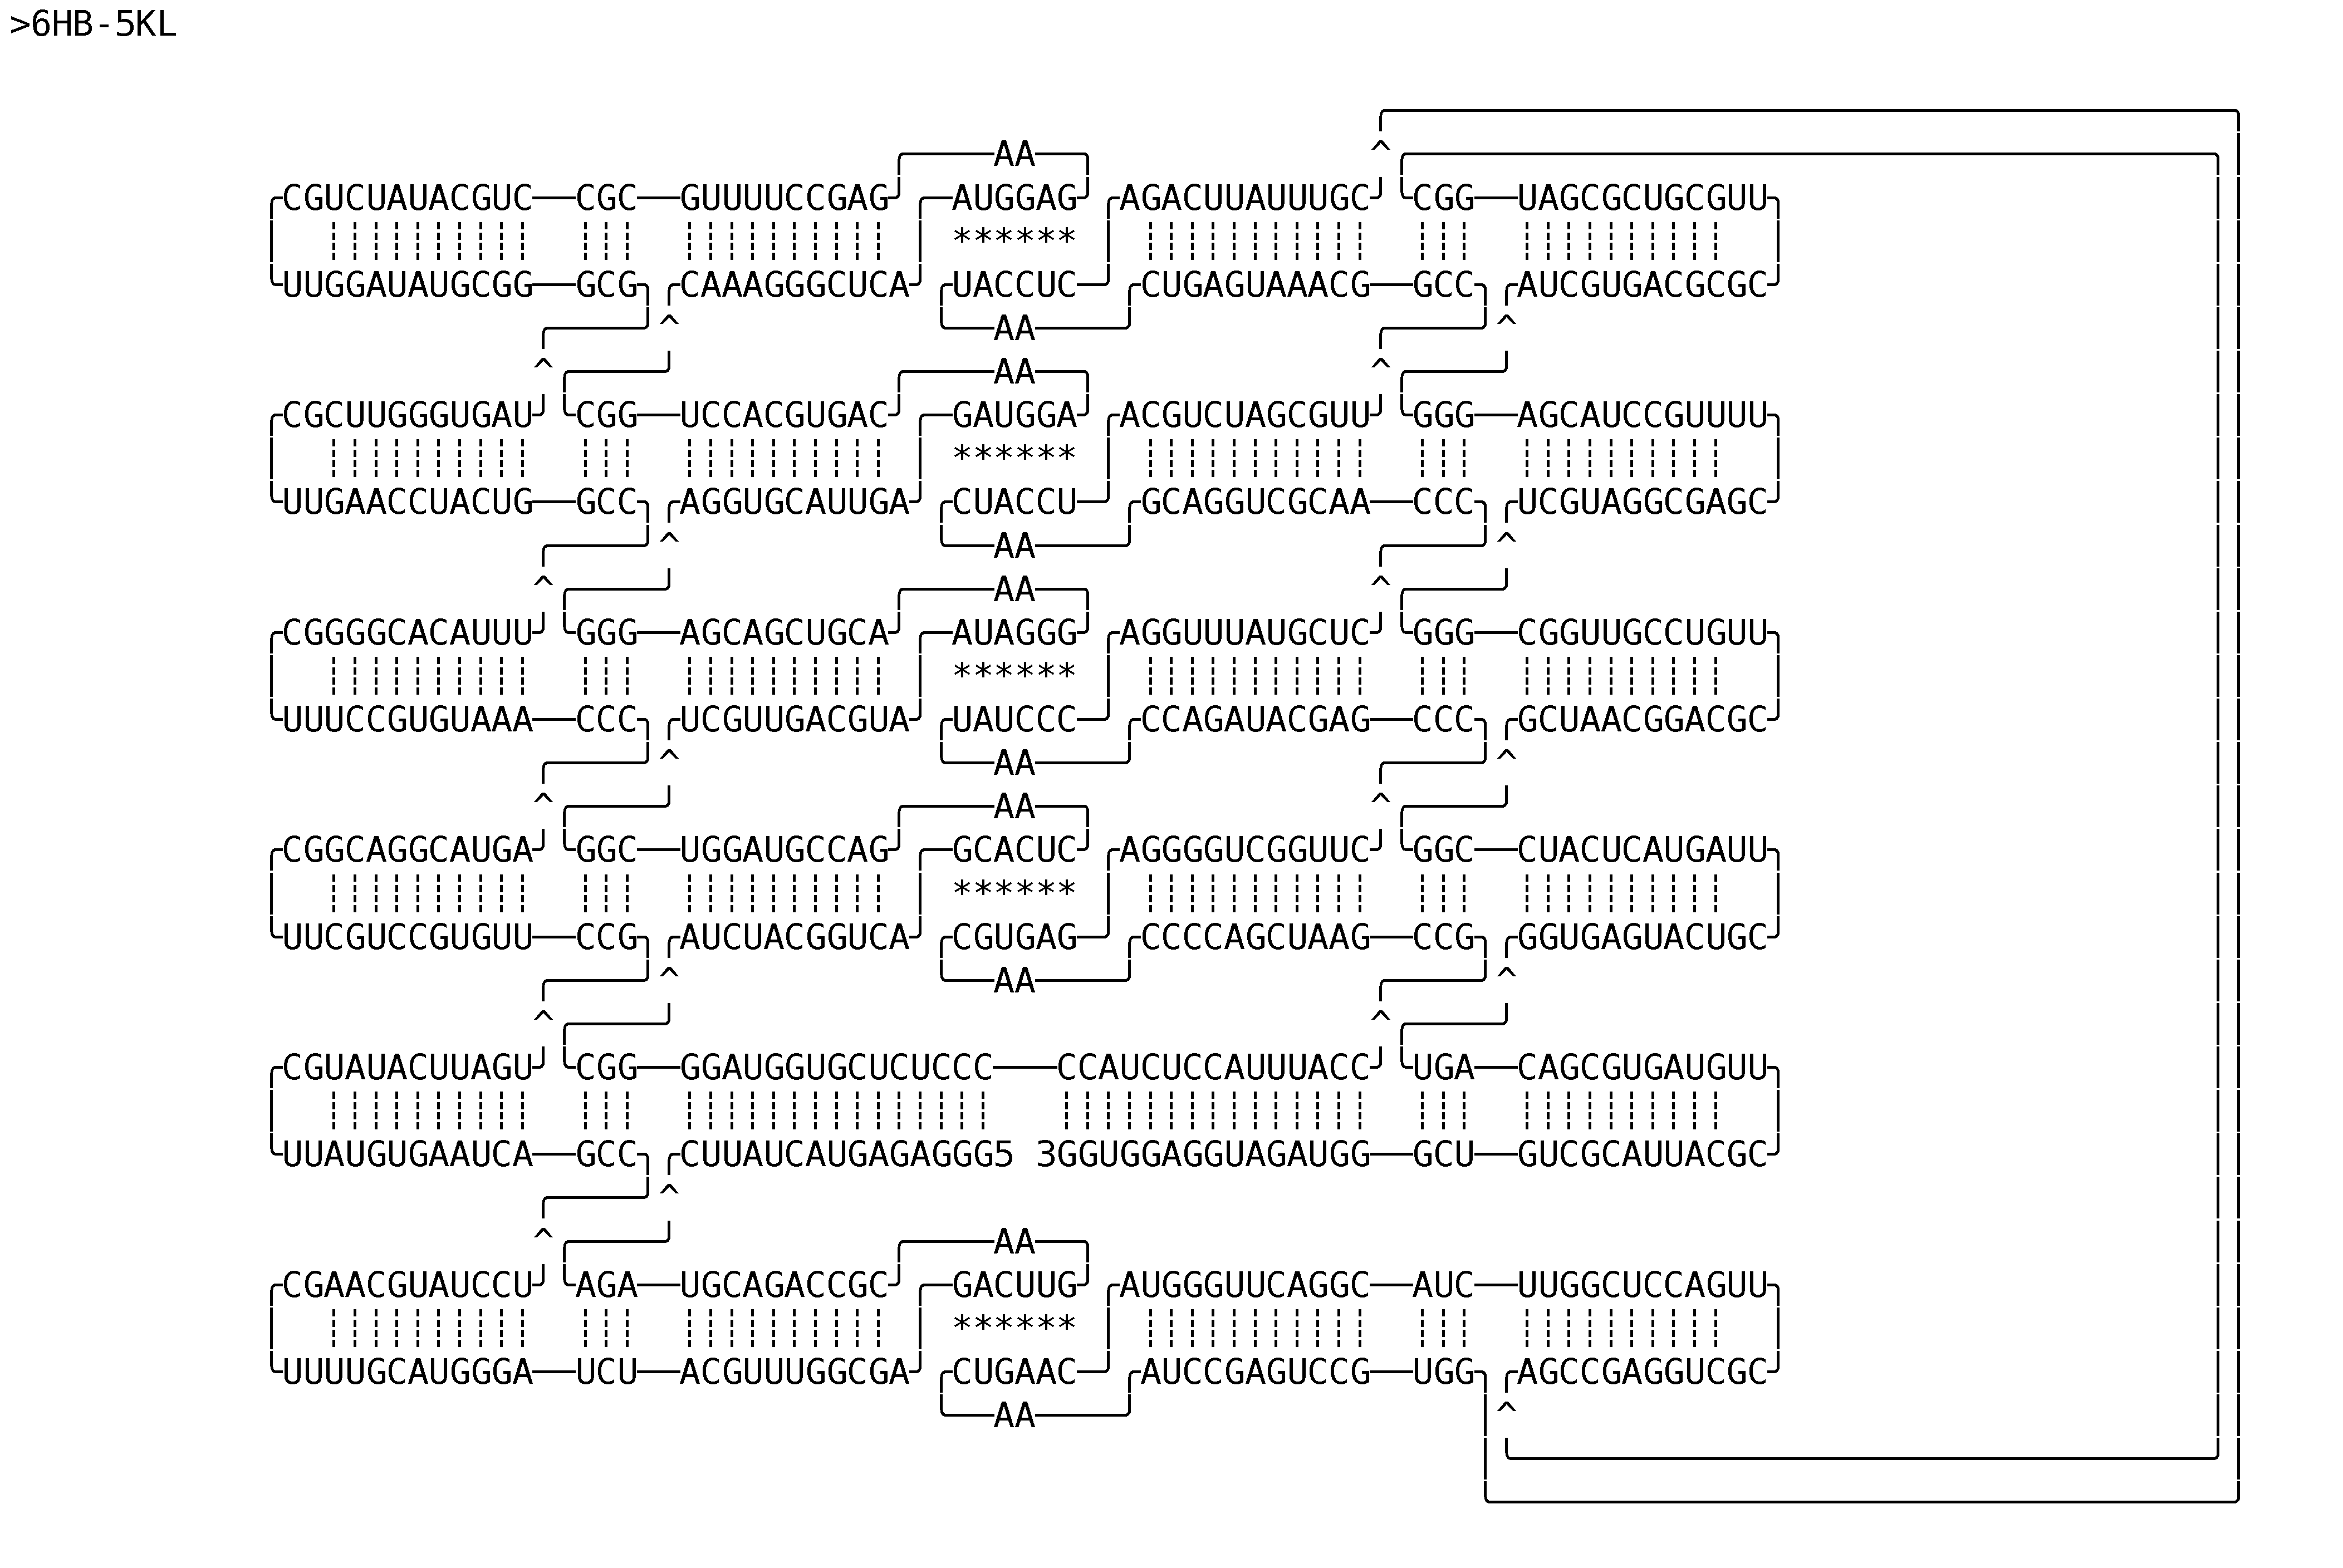
\includegraphics[align=c,width=\textwidth/3]{figures/oxrna_sims/6HB-5KL.eps} \centering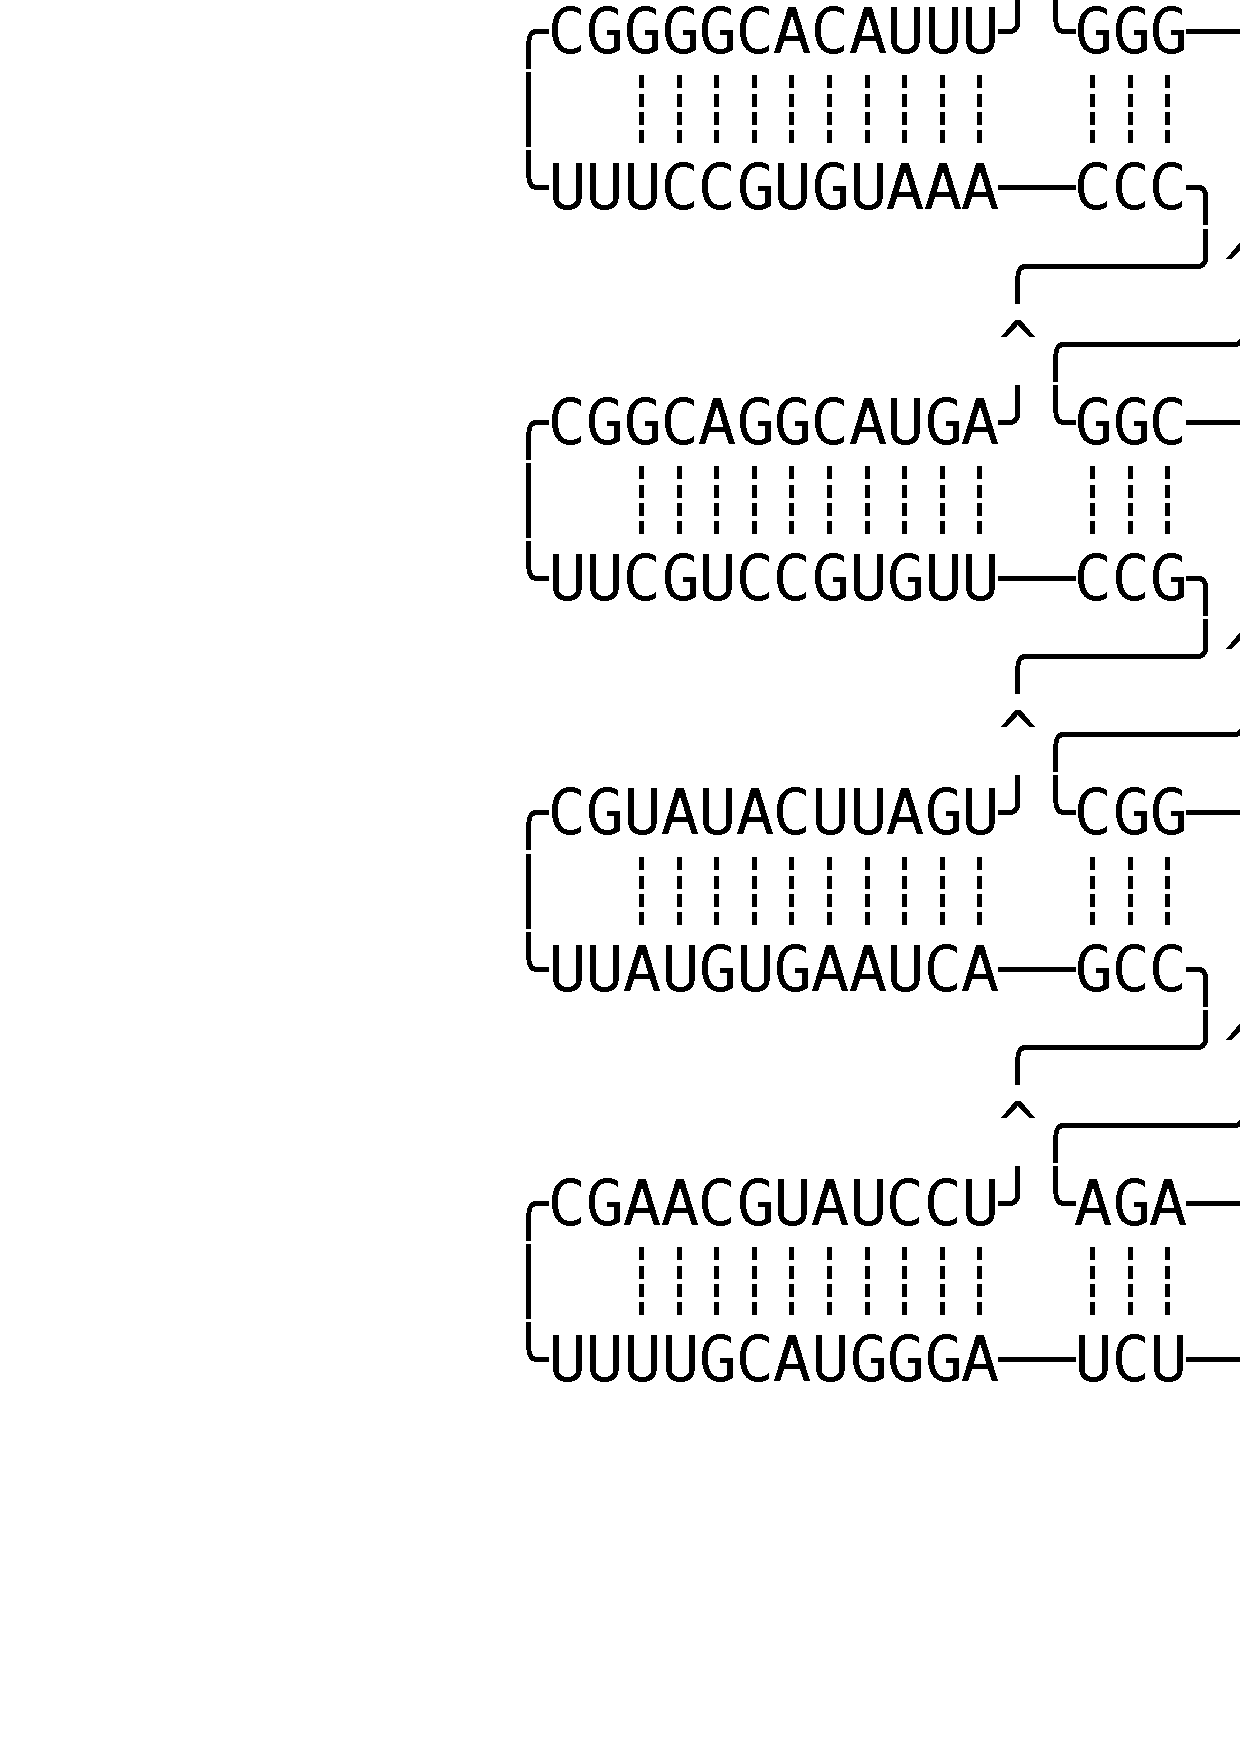
\includegraphics[align=c,width=\textwidth/3]{figures/oxrna_sims/6HB-5KL.png}
  \centering\includegraphics[align=c,width=\textwidth/3]{figures/oxrna_sims/6HB-5KL_last_conf.png}
}
\end{center}
\caption{Conversion and simulation of various RNA designs. Each row, from left to right, shows the ASCII blueprint design, the PDB model (visualised using ChimeraX), and a frame from the simulated structure (visualised using oxView). \textbf{a)} Is a simple hairpin loop. \textbf{b)} is a two-helix bundle tile used in \cite{geary2014single}. \textbf{c)} is two helices connected by a double crossover, analysing the flexibility of such a motif. \textbf{d)} is a possible design for a tensegrity triangle. \textbf{e)} is a siz-helix bundle.}
\label{fig:oxRNA_sims}\end{figure}



